\chapter{Computational Context Through the MRI} \label{chap:compMRI}
This chapter examines the solution to the problem of accretion mentioned in the last section of Chapter~\ref{sec:early}: the MagnetoRotational Instability (MRI). In doing so, it also presents intuition on how the magnetic field interacts in a rotating flow and how the MHD equations outlined in Chapter~\ref{sec:plasmaphysics} actually manifest. Although some traction can be gained analytically (indeed, the instability itself arises from linear theory), this chapter will use simulations to illustrate the linear and nonlinear theory of the MRI and to introduce principles of using numerical simulations. \\
\\
The MRI is fundamentally a local instability; as such, we will zoom in closely to look at a small patch of the overall accretion disk with dimensions $(H,4H,H)$ (see Section~\ref{ssec:shearingbox}) and examine the microphysics at work (see Figure~\ref{fig:global}). The local MHD equations as well as important characteristics such as which wavelengths grow the fastest (and how fast they grow) is outlined in Section~\ref{sec:localideal}. Non-ideal theory and simulations introduce important concepts such as numerical dissipation in Section~\ref{sec:localnonideal}. 
\begin{figure}[h]
  \begin{center}  
    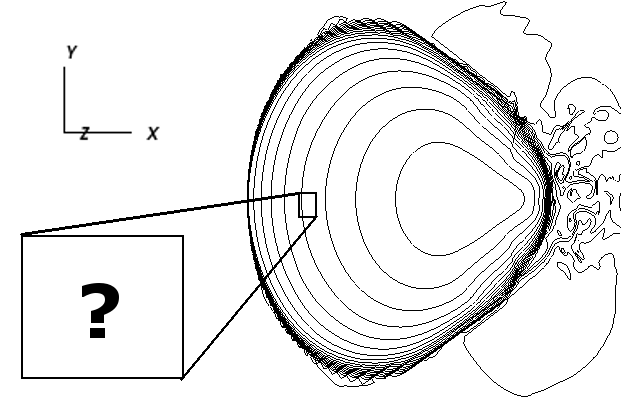
\includegraphics[width=.9\textwidth, angle=0.]{img/global.png}
  \end{center}
  \caption{Global axisymmetric simulation of a hot accretion flow. Such simulations are expensive, so we zoom in to a small box (the ``shearing box'', see Section~\ref{ssec:shearingbox}) to look at the microphysics.}
  \label{fig:global}
\end{figure}

\section{Local Ideal MHD Theory and Simulations} \label{sec:localideal}
In the local approximation, we consider an unperturbed patch of accretion disk with a Keplerian rotation profile at radius $r_0$ threaded by a uniform vertical magnetic field. On such small scales, the patch looks like a rectangular prism. We can write the equations in Cartesian form with the radial direction as $x$ and the azimuthal direction as $y$. The Keplerian differential rotation in this frame looks like a combination of background shear $\vec u_0=2A_0x\hat y$ where $A_0=-3\Omega_0/4$ for Keplerian flow. The ideal MHD equations in this frame are:
\begin{align}
  \nabla\cdot\vec u&=\nabla\cdot\vec B=0\\
  \frac{\partial\vec u}{\partial t}&=-\vec u\cdot\nabla\vec u-\frac1\rho\nabla P+\frac{1}{c\rho}\vec J\times\vec B-2\Omega_0\hat z\times\vec u-4A_0\Omega_0x\hat x\\
  \frac{\partial B}{\partial t}&=\nabla\times\left(\vec u\times\vec B\right)
\end{align}
The second equation incorporates the Coriolis force $-2\Omega_0\hat z\times\vec u$ and the background linear shear~\cite{AST521HW4}. \\
\\
The ultimate goal here is to obtain a relationship between the frequency $\omega$ of a wave perturbation and its wavelength $k$. As such, we consider leading order plane-wave solutions (WKB disturbances) of the form
\begin{align*}
  \vec u&=2A_0x\hat y+\delta\vec ue^{-i(\omega t-kz)} &  \vec B&=B_0\hat z+\delta\vec Be^{-i(\omega t-kz)}
\end{align*}
This form of linear theory is the cornerstone of linear instability analysis in plasma physics and can be found in a number of references~\cite{AST521HW4,BH1998,BH1991a,BH1991b,BH1991c,Quataert2008}. Plugging in this form and eliminating variables, we attain the dispersion relation
\begin{equation}
  \omega^4-\omega^2[\kappa^2+2(\vec k\cdot \vec v_A)^2]+(\vec k\cdot\vec v_A)^2\left((\vec k\cdot \vec v_A)^2+\frac{d\Omega^2}{d\ln R}\right)=0\label{eq:idealdispersion}
\end{equation}
where $\vec v_A=\vec B/\sqrt{4\pi\rho}$ is the Alfven velocity. This equation is also in the Boussinesq limit that the sound speed goes to infinity, which filters out unimportant sound waves~\cite{BH1998,KunzBoussinesq}. 

\subsection{MRI Stability and Maximum Growth Rate}
From the dispersion relation Eq.~\ref{eq:idealdispersion}, we can see the condition for stability (that is, real frequency) is
\begin{equation}
  (\vec k\cdot\vec v_A)^2>-\frac{d\Omega^2}{d\ln R} \label{eq:mriStable}
\end{equation}
It is interesting to note that it is always possible to find a wavenumber $k$ such that the system is unstable unless $\frac{d\Omega^2}{d\ln R}>0$, which would be very uncommon in astrophysical disks~\cite{BH1998}. Thus the MRI is always present in weakly magnetized disks with a Keplerian rotation profile.\\
\\
Also note that if the magnetic field $B=0$, then the Alfven velocity is also zero and Eq.~\ref{eq:mriStable} would have us believe that the hydrodynamic criterion for disk stability is $\frac{d\Omega^2}{d\ln R}>0$. We know however that the Rayleigh linear stability criterion says that $4\Omega^2+\frac{d\Omega^2}{d\ln R}>0$ (outwardly-decreasing specific angular momentum). The disagreement is due to the assumptions made in using the MHD equations, namely, that the mean free path of particles was much less than the length scales of interest. As $k$ increases, we get down to such small scales that the scales of interest become comparable to the mean free path and thus this assumption is no longer valid. The conflict must be resolved through kinetic theory, which is another incentive to investigate the validity of approximating kinetic theory with MHD equations.\\
\\
One of the most important questions for simulations is making sure that the wavelengths that are growing the fastest are resolved on the numerical grid. For this we need the wavelength of the fastest-growing mode, given by taking the derivative of the dispersion relation with respect to frequency. We find that the largest growth rate $\omega_{max}$ is given by
\begin{equation}
  |\omega_{max}|=\frac12\big|\frac{d\Omega}{d\ln R}\big|=\frac34\Omega
\end{equation}
with the Keplerian values on the right. Plugging this back into the dispersion relation shows that the maximimum growth rate occurs when
\begin{equation}
  (\vec k\cdot\vec v_A)^2_{max}=-\left(\frac14+\frac{\kappa^2}{16\Omega^2}\right)\frac{d\Omega^2}{d\ln R}=\frac{15}{16}\Omega^2 \label{eq:idealmaxk}
\end{equation}
There are several interesting things to note here. First, the maximum growth rate is independent of the magnetic field strength or geometry. It is also very large and apparently can grow without bound (although as we will show later other instabilities keep it in check). In fact,~\citet{Balbus1992} suggest that this growth rate is the fastest possible for a linear instability that is powered by the free energy of differential rotation. The fastest-growing wavelength does not change when resistivity is added~\cite{BH1998}. \\
\\
\begin{figure}
  \begin{center}  
    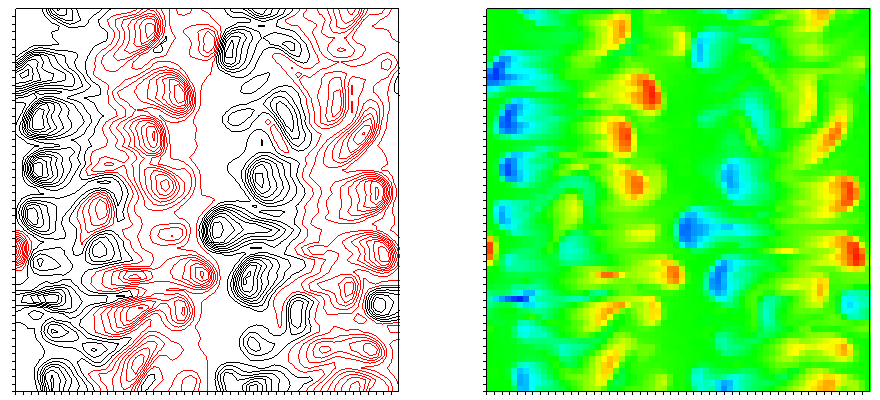
\includegraphics[width=\textwidth, angle=0.]{img/ideal-R1L1-dVy-xz-t30-contpseudo-2.png}
  \end{center}
  \caption{Slice at $t=3.0$ orbits. Central body is on the left; z-direction is up. Plots are normalized to initial pressure. Left: Contour plot of twenty azimuthal angular momentum perturbation levels. Black is a perturbation in the negative y-direction (which means falling radially in), while red is in the positive y-direction. Right: Pseudocolor plot of azimuthal angular momentum perturbations. The growth of the x-direction mode with wavelength .5H is clear. Also see Section~\ref{ssec:shearingbox}.}
  \label{fig:idealgrowth}
\end{figure}
\begin{figure}
  \begin{center}  
    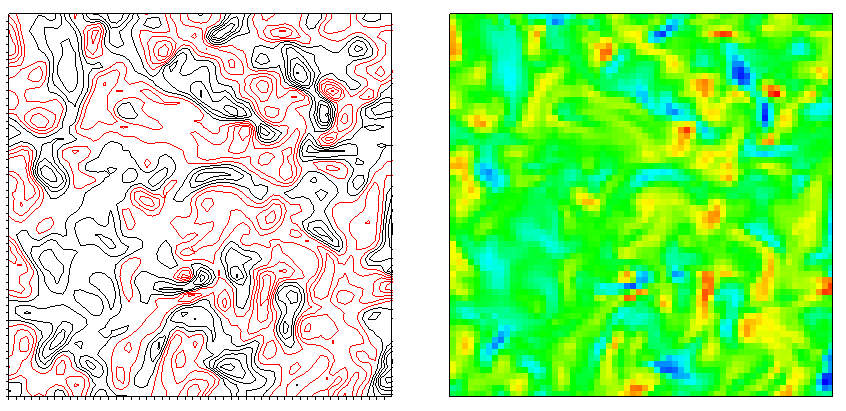
\includegraphics [width=\textwidth, angle=0.]{img/ideal-R1L1-01-dVy-xz-t49-2.png}
  \end{center}
  \caption{Slice at $t=4.9$ orbits of azimuthal angular momentum perturbations (see Fig.~\ref{fig:idealgrowth}). The system has proceeded to the nonlinear turbulence phase as evidenced by the lack of structure. Also see Section~\ref{ssec:shearingbox}.}
  \label{fig:idealturb}
\end{figure}
We can see this growth in action by examining Figure~\ref{fig:idealgrowth}, which plots perturbations in azimuthal angular momentum for a small patch of the accretion disk (see Section~\ref{ssec:shearingbox}). There is clearly a periodic structure which in the x-direction has a wavelength of about half of the box size. This is what we expect from Eq.~\ref{eq:idealmaxk}:
\begin{align*}
  (\vec k_{max}\cdot \vec v_A)^2&=k_{max}^2\frac{B^2}{4\pi\rho}=\frac{k_{max}^2}{4\pi\rho}\frac{8\pi P}{\beta}=\frac{2P}{\beta\rho}k_{max}^2=\frac{15}{16}\Omega^2
\end{align*}
With the parameters of the simulation having been chosen to set $\Omega=1$, $P/\rho=1$, and $\beta=400$, we have $k_{max}=13.7~H^{-1}$ in units of the computational box size $H$. The wavelength of the fastest growing mode is then $\lambda_{max}=.46H$. The figure shows this and its orientation along the x-direction. The z-direction mode has a different growth rate and wavelength. In all simulations in this thesis, the magnetic field is given as $\vec B=B_0\sin\left(\frac{2\pi x}H\right)\hat z$. This choice is significant only in that it has zero net flux; the actual form as a sine wave is somewhat arbitrary as it is just a simple way to achieve zero net flux.\\
\\
More detailed analysis of the instability can be found in~\citet{BH1991a,BH1991b,BH1991c,BH1998}, the last of which will henceforth be referred to as~\citetalias{BH1998}. The instability is different given different initial configurations of the magnetic field, the most important being the aforementioned zero net-flux condition. A radial magnetic field component will yield a time-dependent azimuthal magnetic field component; however, this dependency does not really affect the MRI evolution because the axisymmetric instability is independent of $B_\phi$~\cite{BH1998}. \\
\\
The magnetic energy and kinetic energy increase when the MRI is in action because some of the (in this case, unlimited) energy from differential rotation is going into turbulence, sustaining the magnetic field and churning around particles. The linear phase of the MRI in Figure~\ref{fig:idealgrowth} gives way to turbulence shortly thereafter, as shown in Figure~\ref{fig:idealturb}. The nonlinear regime is the steady-state solution and is what we are most interested in for this thesis. This is the regime that is difficult to describe analytically. The ``channel mode'' bump that dominates in two dimensions~\cite{BH1991a} breaks down much faster in three dimensions~\cite{HGB1995,HGB1996}, as seen in Section~\ref{sec:localnonideal}.

%---------------------------------------------------------------------%
\subsection{Spring Interpretation}\label{ssec:springs}
It turns out that the local equations are also those of two orbiting masses coupled by a spring. A more complete derivation is given in~\citetalias{BH1998}, so here we only provide the physical intuition for how the MRI leads to accretion. \\
\\
The situation is illustrated in Figure~\ref{fig:springs}. One mass (call it $m_o$) is orbiting at a slightly higher-radius orbit $r_o$ thanks to a perturbation. Due to the Keplerian rotation law, this mass orbits slower than the mass $m_i$ at lower radius $r_i$. This means that $m_i$ pulls ahead of $m_o$, thus stretching the spring. Hooke's law exerts a force pulling the springs back together, causing the inner mass to lose angular momentum and the outer mass to gain angular momentum. This means that $m_i$ drops down to a lower orbit while $m_o$ pulls away, thereby stretching the spring even more. The process runs away and $m_i$ falls inward while $m_o$ falls outward, producing outward angular momentum transport. \\
\\
Obviously there is not an actual spring connecting the two masses. The job of the spring's restoring force is done by magnetic tension $\left(\frac{1}{4\pi}(\vec B\cdot\nabla)\vec B\right)$, which tries to unfurl magnetic field lines. Due to flux-freezing, the magnetic field is distorted when the fluid elements are perturbed. The field line is drawn as a dotted orange line in Figure~\ref{fig:springs}.
\begin{figure}
  \begin{center}  
    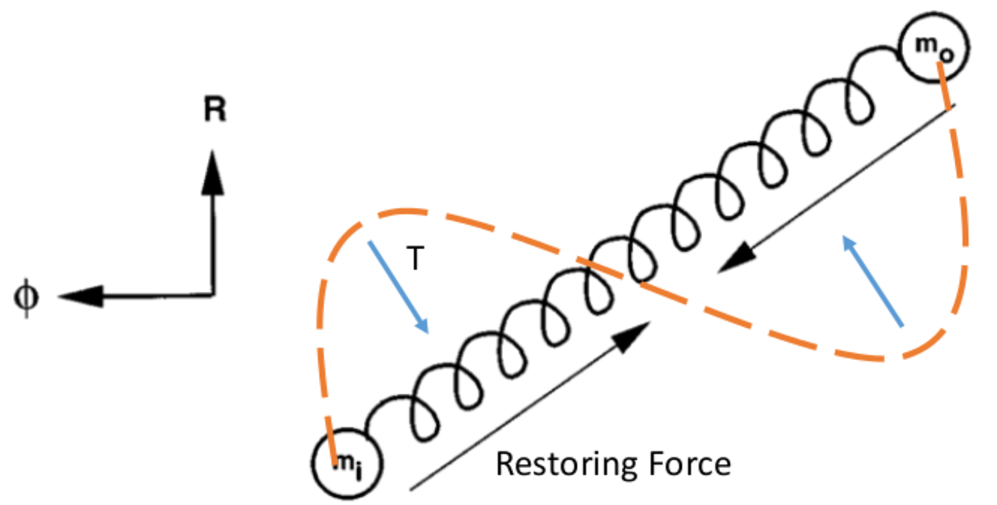
\includegraphics[width=.8\textwidth, angle=0.]{img/mriSpring.pdf}
  \end{center}
  \caption{Illustration of the MRI with the magnetic tension $T$ working in the same way as the restoring force of a spring. Adapted from~\citetalias{BH1998}.}
  \label{fig:springs}
\end{figure}
%
%
\subsection{Shearing Box Method}\label{ssec:shearingbox}
The shearing box method examines a small enough region of a system that stratification and curvature can be neglected, which means that results of shearing-box simulations are applicable to a broad range of flows~\cite{Walker2017}. The shearing-box approximation solves the Cartesian set of MHD equations described above with periodic boundary conditions. The model's linear shear means that if a particle moves outward with radius, it also moves azimuthally. The boundary conditions for a function $f$ are expressed as
\begin{align}
  f(x,y,z)&=f(x+H_x,y+\frac32\Omega_0H_xt,z)\label{eq:bcx}\\
  f(x,y,z)&=f(x,y+H_y,z)\label{eq:bcy}\\
  f(x,y,z)&=f(x,y,z+H_z)\label{eq:bcz}
\end{align}
where the first line is for the x boundary, the second for the y boundary, and the third for the z boundary. The size of the computational regime is $H_x=H$ in the x-direction, $H_y=4H$ in the y-direction, and $H_z=H$ in the z-direction. In these equations the shear has been Taylor-expanded about the relative velocity $w_y=v_y-R\Omega_0=R(\Omega-\Omega_0)\sim x\left(R\frac{d\Omega}{dR}\right)_0=-\frac32\Omega_0x$ for a Keplerian disk. These boundary conditions are visually explained in Figure~\ref{fig:shearingbox}. More details can be found in~\citetalias{BH1998} or in the first paper simulating the MRI~\cite{BH1991c}. \\
\\
Since the box is in the local approximation, we can take the density and pressure to be initially constant. In this thesis, we evolve the system adiabatically as opposed to isothermally as discussed in Chapter~\ref{sec:idealMHD}. We also choose units such that the fiducial angular velocity of the shearing box as it goes around the central body is 1: $\Omega_0=1$. Also choosing $P=\rho=1$, we have that the sound speed $c=1$ and thus that the disk height $H=1$. \\
\\
Finally, note the importance of resolution: if the fastest growing MRI mode is smaller than the size of each zone, then the simulation will not resolve the mode and the set-up will appear stable. Calling the size of each zone $(\Delta x,\Delta y,\Delta z)$, the smallest resolvable wavelength in the x-direction is
\begin{equation*}
  \lambda_{min}=2\Delta x
\end{equation*}
This paper's simulations run with $64x128x64$ zones on Della and $64x197x64$ on Perseus. Each zone has a size $\Delta x=1/64~[H]$ and the smallest wavelength we can see corresponds to $\lambda_{min}=1/32~[H]\approx.03~[H]$. We need the fastest growing wavelength to be bigger than this in order to see turbulence.
\begin{figure}[h]
  \begin{center}  
    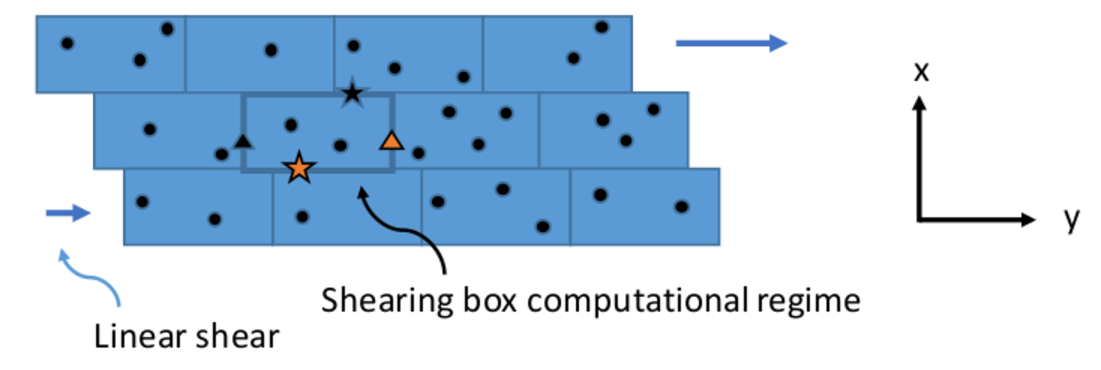
\includegraphics [width=\textwidth, angle=0.]{img/ShearingBox.pdf}
  \end{center}
  \caption{Illustration of the shearing box method. The computational regime itself is outlined in thick blue (``shearing box computational regime'') and has dimensions of $H_x=H$, $H_y=4H$, and $H_z=H$ (z dimension not shown). The azimuthal direction needs a larger computational domain because the shear stretches the modes out. The linear shear $\vec u_0=2A_0x\hat y$ is illustrated by arrows that vary in size with the x-location. The boundary conditions of Eqns.~\ref{eq:bcx}-\ref{eq:bcz} are shown by the orange and black triangle and star. A particle that travels off the right (y) boundary (orange triangle) reappears on the left y boundary at the same x-position, represented by the black triangle. The x boundary condition takes into account the linear shear, such that the orange star leaving through the x boundary reappars displaced as though by a shear at the top of the regime (black star). Adapted from~\citetalias{BH1998}.}
  \label{fig:shearingbox}
\end{figure}

%--------------------------------------------------------------%

\section{Local Non-ideal MHD Theory and Simulations} \label{sec:localnonideal}
This section is particularly relevant for the next chapter and understanding the effects of changing resistivity and viscosity in a fluid model. When we introduce non-ideal MHD components such as resistivity and viscosity, the resolution of simulations becomes even more important. This is because certain length scales are damped faster than others. A problem in the literature involving the lack of convergence for zero net-flux simulations such as these was recently resolved~\cite{Fromang2007a,Shi2016,Walker2017}. These papers found that in order to sustain turbulence, the box size must be larger in the vertical direction. Since the box size of this thesis is smaller in the vertical direction, we can expect some wavelengths to be cut off and therefore a minimum magnetic Prandtl number of 4 is required to sustain turbulence~\cite{Fromang2007b,Simon2009a} (the case is different for net-flux simulations~\cite{Simon2009b}).\\
\\
As a rough estimate, resistivity has a characteristic wavelength $k^2\eta\sim\Omega$ that is damped by $1/e$ over the time it takes for a sound wave to traverse the disk. Too big a value will damp the MRI and stabilize the disk~\cite{Fleming2000}. Viscosity similarly damps wave numbers $k^2\nu\sim\Omega$. The balance between these two competing scales means that there is a limited parameter space in magnetic Prandtl number that can be explored. Requiring that the resistivity be large enough to damp the smallest resolvable wavelength and small enough not to damp the fastest-growing mode leads to a possible range of resistivities
\begin{equation*}
 \num{2.5e-5}<\eta<\num{5e-3}
\end{equation*}
The same bound applies for the viscous transport coefficient $\nu$.\\
\\
A set of simulations with $\eta=\num{1e-4}$ is shown in Figure~\ref{fig:nstokesPm}a) with varying magnetic Prandtl number. We can see that magnetic energy increases with increasing $Pm$. However, Figure~\ref{fig:nstokesPm}b) shows that increasing $Pm$ does not monotonically lead to increasing magnetic energy. This decay is due to the viscous damping of more modes, since at for example $Pm=12$, $\nu=\num{24e-4}$ which is getting close to damping the fastest-growing mode. In such cases, the flow will not be turbulent and so the magnetic energy will decay. Note that Figure~\ref{fig:nstokesPm}b) has a lower overall magnetic energy because the dissipation due to both resistivity and viscosity is greater.
%
\begin{figure}[h]
  \begin{center}  
    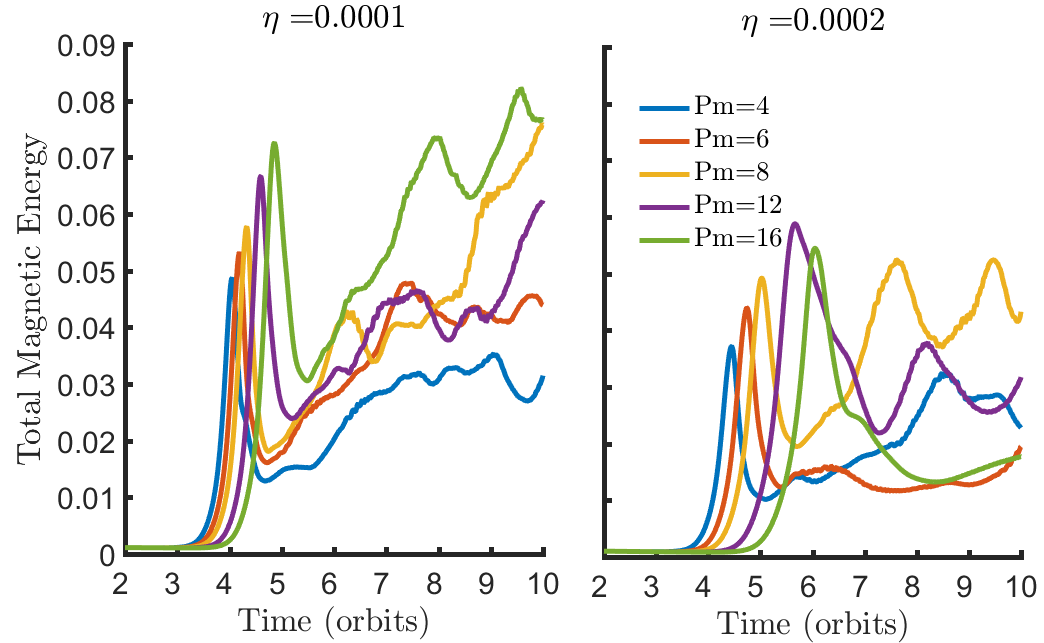
\includegraphics [width=\textwidth, angle=0.]{img/eta1-2-PmME16.png}
  \end{center}
  \caption{Plots of magnetic energy with increasing magnetic Prandtl number. The left panel has $\eta=\num{1e-4}$ and the right has $\eta=\num{2e-4}$. For the lower resistivity, magnetic energy increases monotonically up to $Pm=16$. For a higher resistivity however, viscous damping begins to stabilize the MRI and higher $Pm$ result in a decrease of  magnetic energy.}
  \label{fig:nstokesPm}
\end{figure}
%
